\documentclass[../rzero]{subfiles}
\begin{document}
\chapter{Monopole Gravitational Waves}\label{monopoleGravitationalWavesChapter}

\begin{chapquote}{Eric Weinstein talking to Brian Keating, \textit{Youtube\cite{drbriankeatingEricWeinsteinTheoretical2020}}}
``You guys need more money. You struck the worlds worst licening deal.''
\end{chapquote}

\section{Monopole Waves}
Monopole Waves are waves that emanate spherically from a source. Due to symmetry, they can really only be pressure, also known as longitudinal waves. The typical example is a spherical speaker (who has spherical speakers?) turned on. The sound (sound is a pressure wave) goes in all directions and each wave crest forms a spherical pattern, moving away from the speaker at the speed of sound. 

\section{They Can't Exist}
One of the most famous theorems of General Relativity is Birkoff's Theorem\cite{Birkhoff1923}. It's clear, the gravitational field outside a spherical mass is always exactly the static Schwarschild field. So with that big word static in there, it seems there cannot be and monopole gravitational waves. Case closed. 

One can, however, make (an almost trivial) 'dragged along' monopole gravitational wave by imagining a typical supernova explosion, with an (unlucky) observation spacecraft orbiting around it. The basics are depicted in figure (\ref{monopoleFigure}) In a supernova a large amount of energy is emitted as neutrinos as the first step, about 1/1000 of a solar mass worth of energy. The spaceship has no decent neutrino detector on board, but can of course observe its own motion accurately. It will notice the central mass drop. This wave (not self supported), is a monopole $p-wave$, it's spherically symmetric, and will bend a ring of beads in manner so as to allow the extraction of energy (Feynman's criteria).  


\subsection{Vacuum solution}
Another example of this phenomenon is looking at a typical LIGO\cite{collaborationGW150914FirstResults2016} like this using the vacuum Einstein Equations. In that case 5\%, or 3 solar masses of energy passed by our unlucky satellite. It's interesting to think about this monopole wave as a necessary part of even the vacuum field equations. In linearized General Relativity there is no accompanying monopole 'depression' under a wave packet, leading to the common belief that the gravitational field contains no energy. It's more than a belief though, as the vacuum Einstein equations have no term for the self field energy. It may be that the Einstein theory of General Relativity is missing something!\cite{08092323EnergyMomentumGravitational}. See chapter \ref{energyGeneralRelativityChapter} - where I look at this in depth. 

\begin{figure}\label{monopoleFigure}
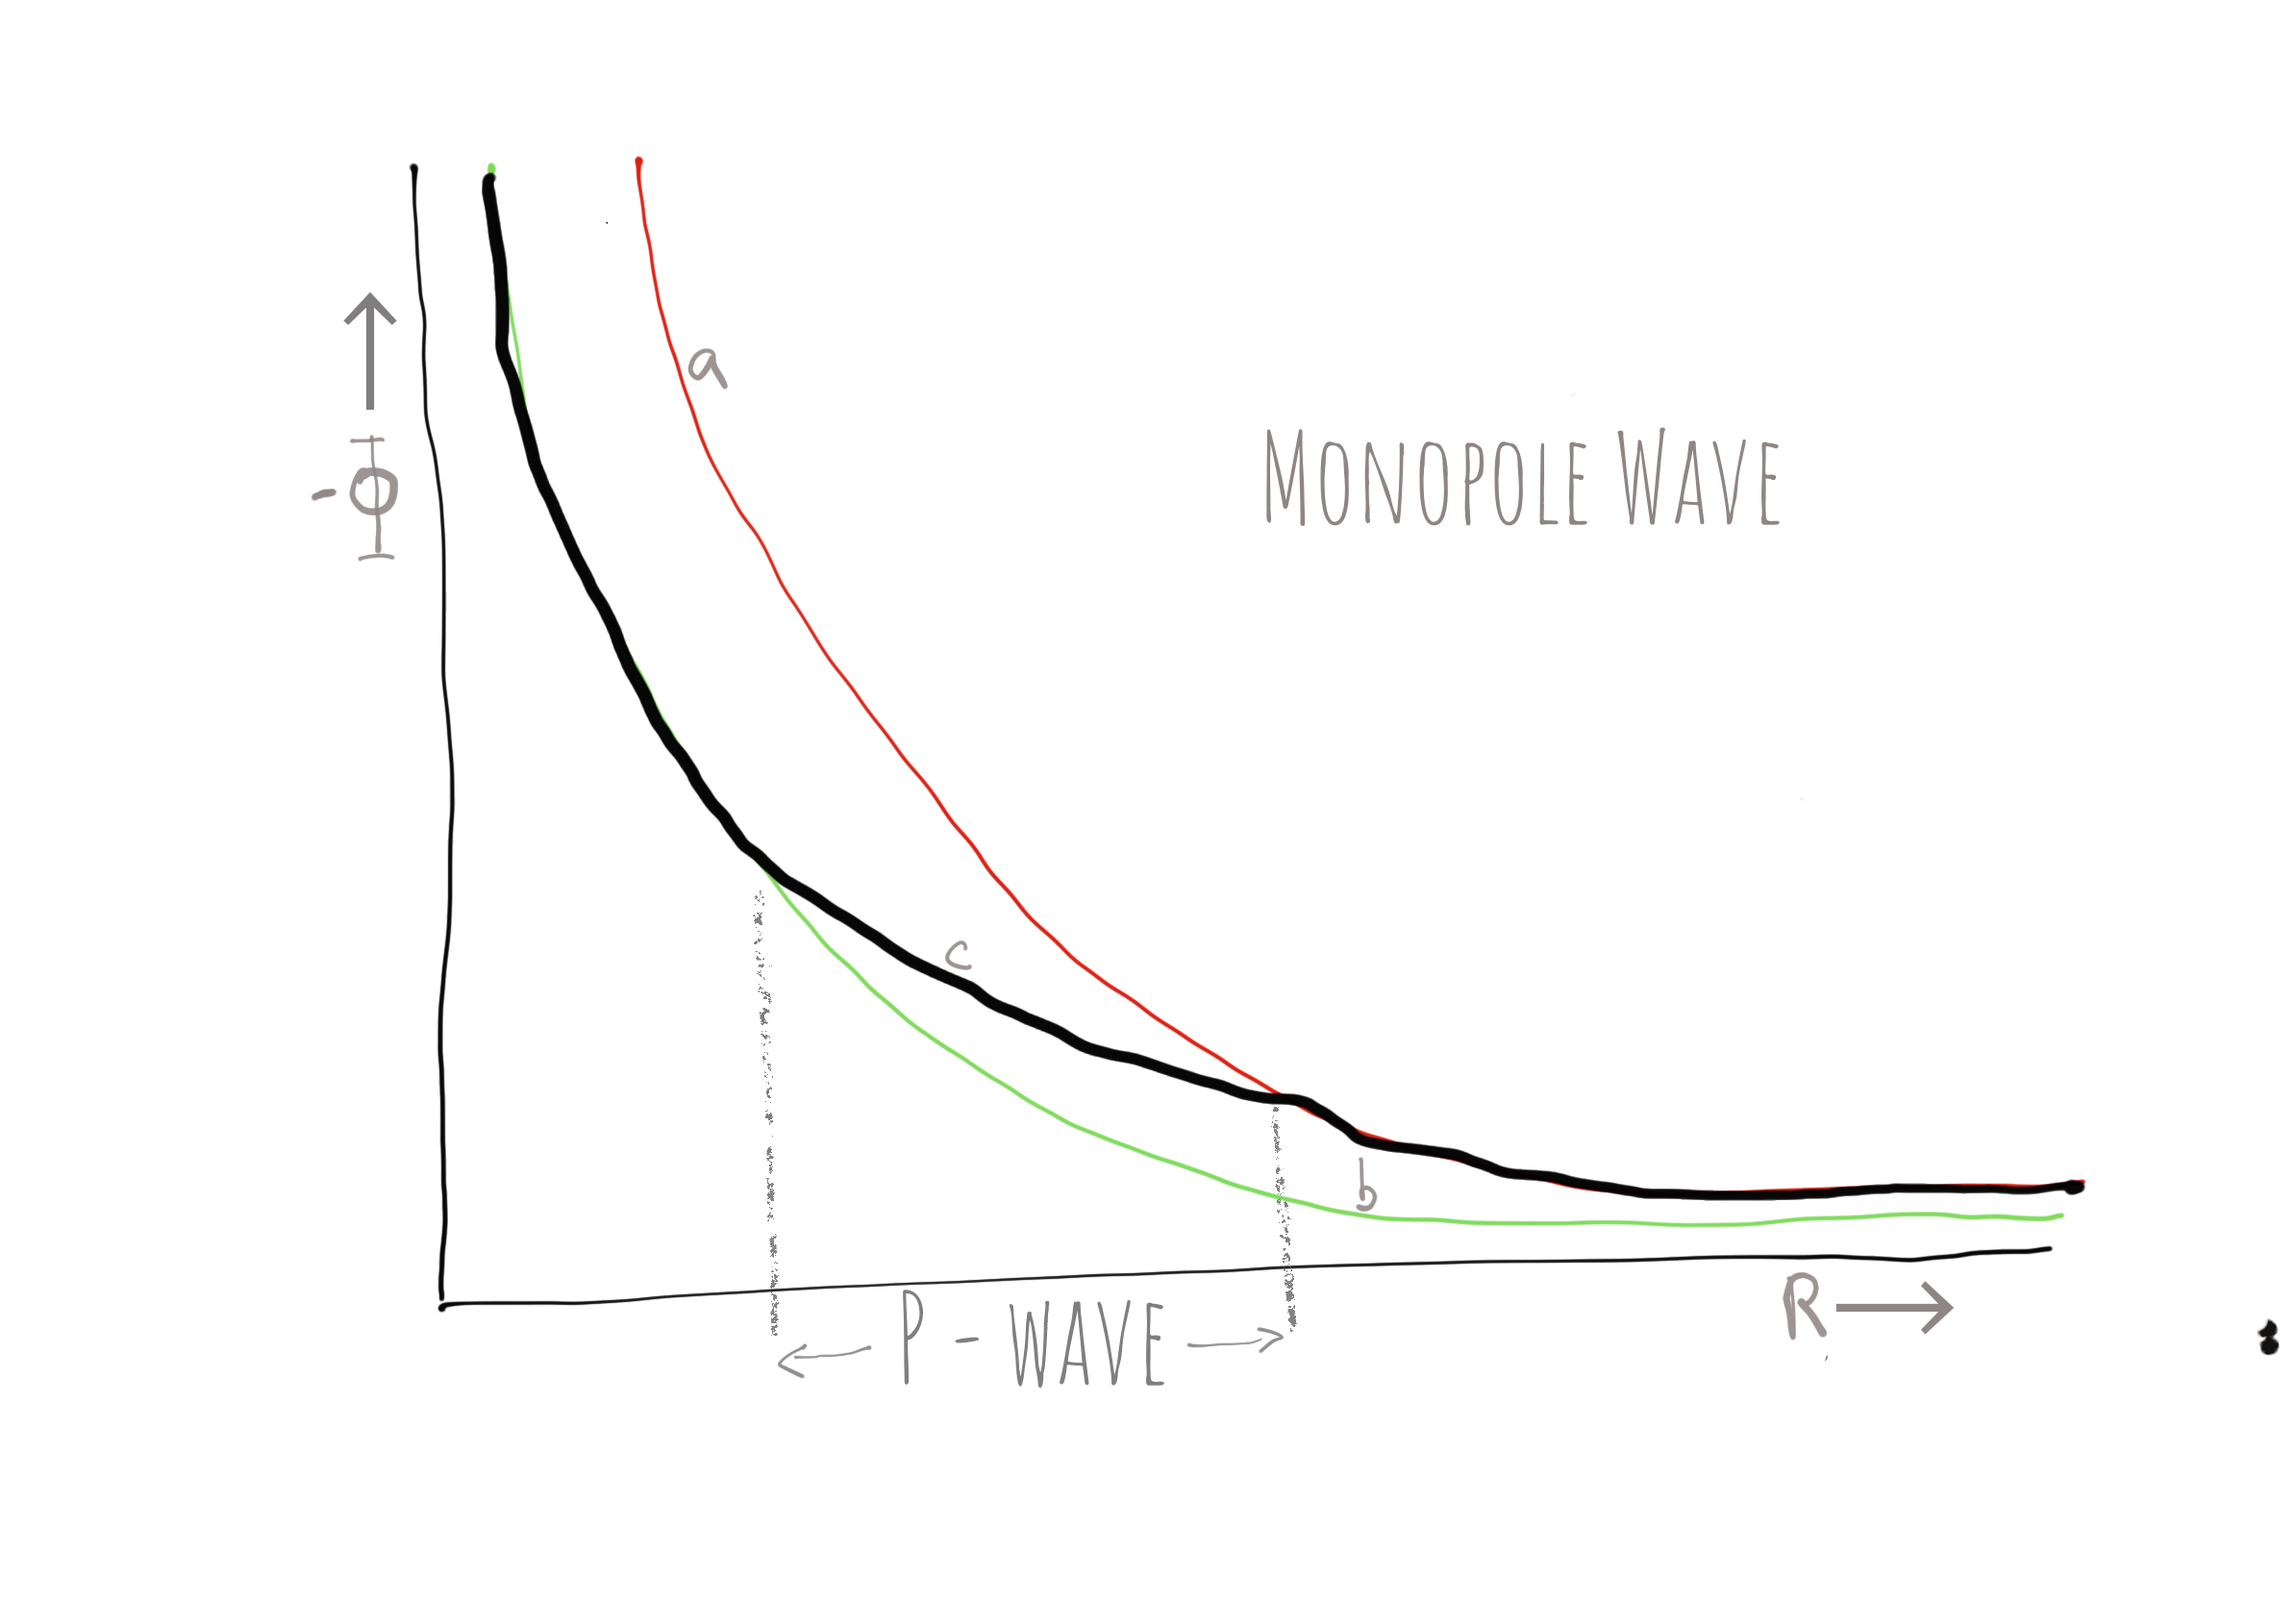
\includegraphics[width=\textwidth]{chapters/images/monopole.png}
\caption{Monopole Wave: Birkhoff's theorem holds even for a dynamic situation as, for instance discussed in the text. The left axis is the negative of the gravitational potential, bottom axis is radius. Curve $a$ is for a large mass, $b$ for a small mass, and $c$ for the actual physics. The region shown by the label $P - Wave$ is the location of the moving monopole gravitational wave.}
\end{figure}






\section{Energy argument for their existence}

\subsection{Velocity of Monopole Waves}
	Like $\num{10e4} c$ 

\section{With Einsteins }

\section{Assuming Chapter \ref{energyGeneralRelativityChapter} Works}
	refer heavily back to chapter \ref{energyGeneralRelativityChapter}. Maybe quote some stuff on other theories of gravity having monopole 

\section{Experimental Findings}
Faster than light collapse



\section{Quantum Mechanics from General Relativity}
my theory


\section{Dark matter is quantum mechanics}
	Model is laid out 
\end{document}
